\documentclass{article}
\usepackage[utf8]{inputenc}
\usepackage[margin=0.35in]{geometry}


\title{Computer Networks Lab 5}
\author{Shane Cincotta }
\date{April 17, 2020}

\usepackage{natbib}
\usepackage{graphicx}

\begin{document}

\maketitle

\begin{figure}[h!]
\centering
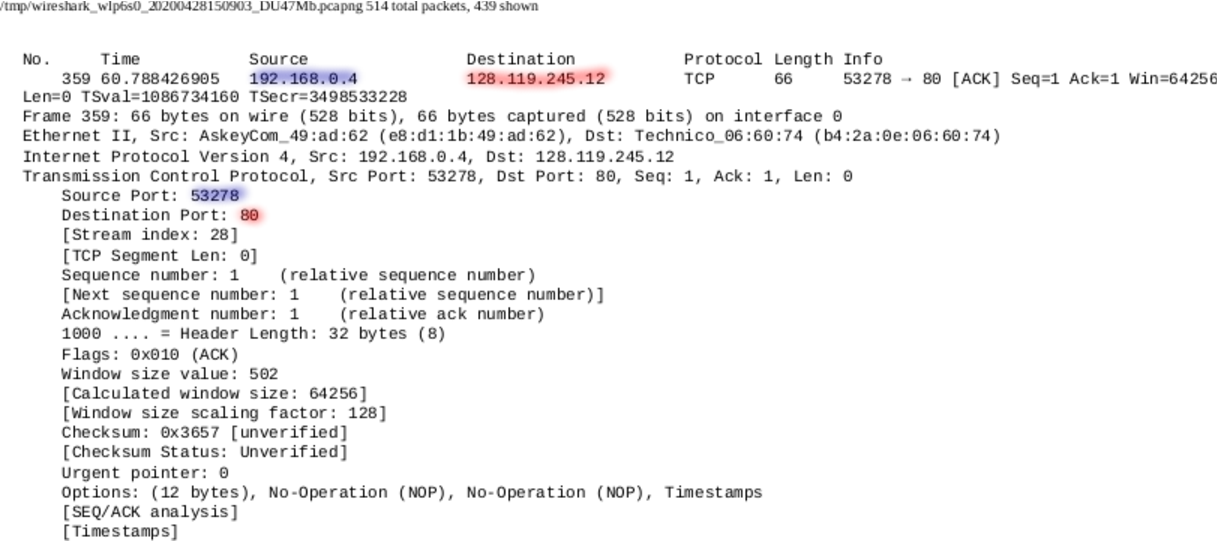
\includegraphics[scale=0.5]{Q1-3.pdf}
\caption{IP address and TCP port number used by the client computer}
\end{figure}

\section*{1}
What is the IP address and TCP port number used by the client computer (source)
that is transferring the file to gaia.cs.umass.edu?\\
\newline According to figure 1, the IP address is 192.168.0.4 and the port number is 53278.\\

\section*{2}
What is the IP address of gaia.cs.umass.edu? On what port number is it sending
and receiving TCP segments for this connection?\\
\newline According to figure 1, the destination IP is 128.119.245.12 and the destination port is 80.\\
\section*{3}
What is the IP address and TCP port number used by your client computer
(source) to transfer the file to gaia.cs.umass.edu?\\
\newline According to figure 1, the IP address is 192.168.0.4 and the port number is 53278.\\
\clearpage
\section*{4}
What is the sequence number of the TCP SYN segment that is used to initiate the
TCP connection between the client computer and gaia.cs.umass.edu? What is it
in the segment that identifies the segment as a SYN segment?\\
\newline According to figure 2, the sequence number of the TCP SYN segment that is used to initiate the TCP connection is 0.  This segment is identified by the SYN tag being set to 1.\\
\begin{figure}[h!]
\centering
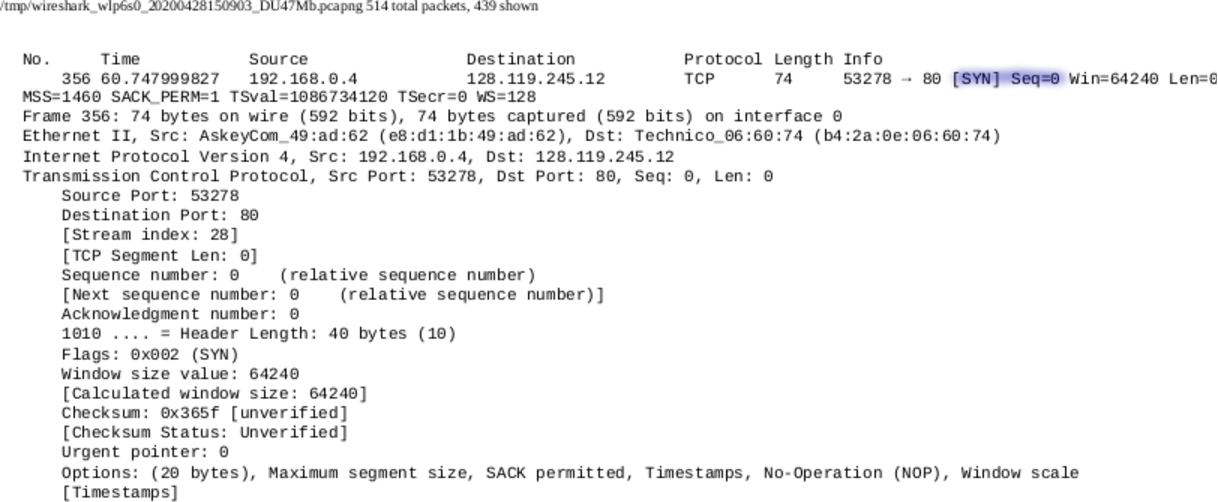
\includegraphics[scale=0.5]{Q4.pdf}
\caption{TCP SYN segment that is used to initiate the TCP connection}
\end{figure}
\section*{5}
What is the sequence number of the SYNACK segment sent by gaia.cs.umass.edu
to the client computer in reply to the SYN? What is the value of the
Acknowledgement field in the SYNACK segment? How did gaia.cs.umass.edu
determine that value? What is it in the segment that identifies the segment as a
SYNACK segment?\\
\newline According to figure 3, the sequence number of the SYNACK segment sent by gaia.cs.umass.edu
to the client computer is 0.  The value of the ACK is 1.  This number is determined by adding 1 to the initial sequence number of the SYN segment from the client to the computer.  The SYN flag and ACK flag are set to 1 and they indicate that this segment is an SYNACK segment.\\
\begin{figure}[h!]
\centering
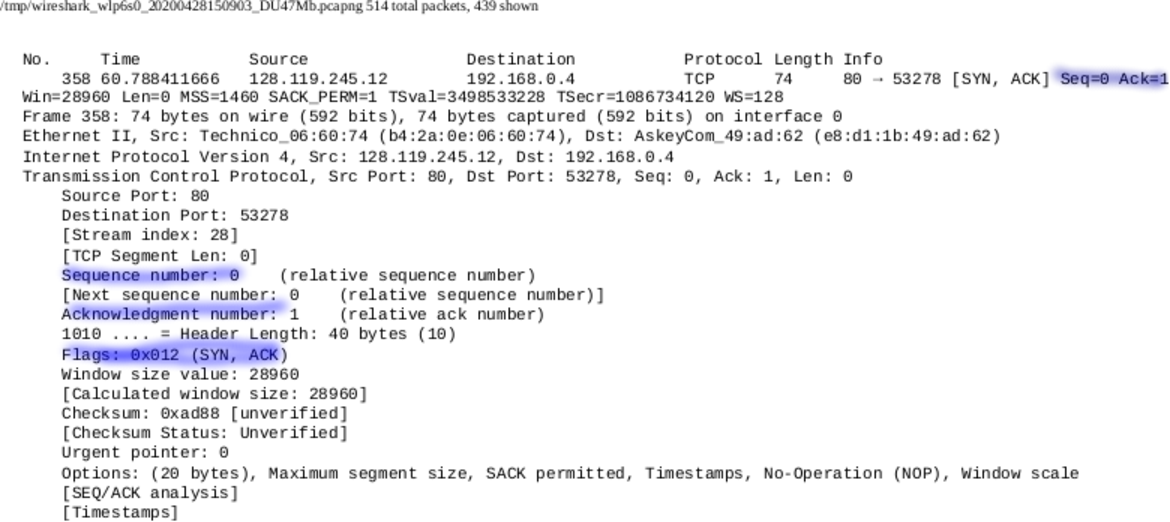
\includegraphics[scale=0.5]{Q5.pdf}
\caption{SYNACK segment sent by gaia.cs.umass.edu}
\end{figure}
\clearpage
\section*{6}
What is the sequence number of the TCP segment containing the HTTP POST
command?\\
\newline According to figure 4, the sequence number of the TCP segment containing the HTTP POST
command is 149145.\\
\begin{figure}[h!]
\centering
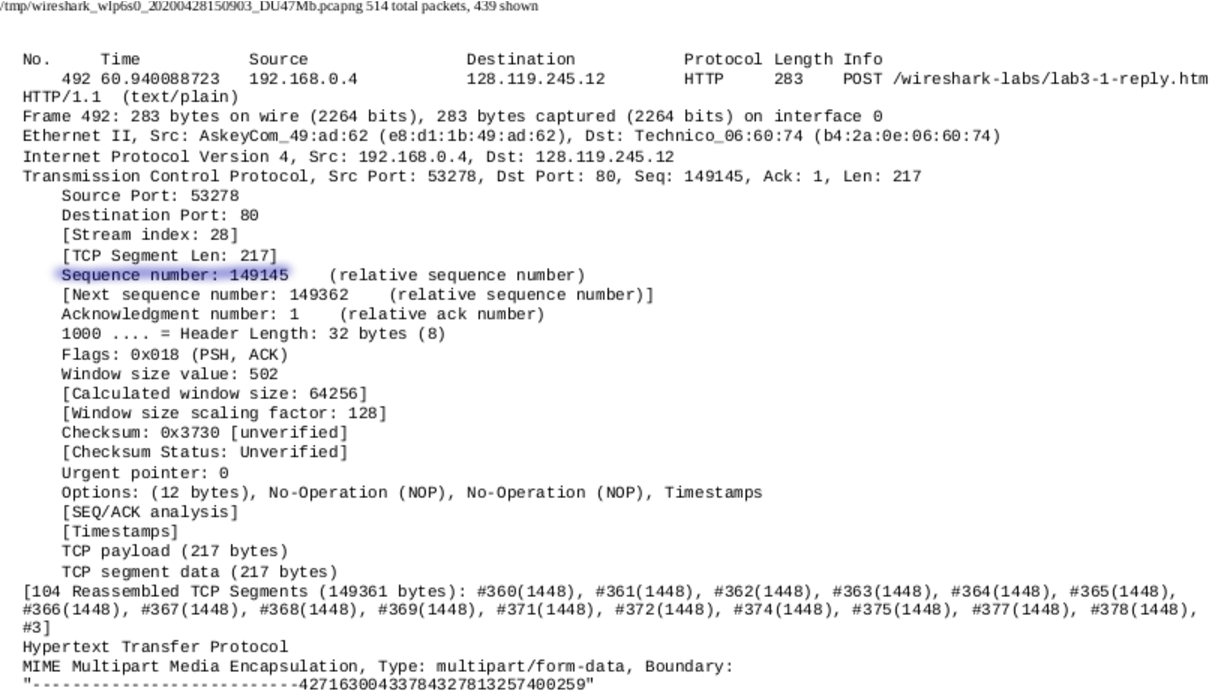
\includegraphics[scale=0.5]{Q6.pdf}
\caption{Sequence number of the TCP segment containing the HTTP POST
command}
\end{figure}
\section*{7}
Consider the TCP segment containing the HTTP POST as the first segment in the
TCP connection. What are the sequence numbers of the first six segments in the TCP connection (including the segment containing the HTTP POST)? At what
time was each segment sent? When was the ACK for each segment received? Given the difference between when each TCP segment was sent, and when its acknowledgement was received, what is the RTT value for each of the six segments? What is the EstimatedRTT value after the receipt of each ACK?\\
\newline According to figure 5, the sequence numbers of the first 6 segments are 1, 579, 716, 2164, 3612, 5060.  Figure 6 shows the send time, received (ACK) time and RTT.\\
\newline The required formula is $EstimatedRTT_s = 0.875 * EstimatedRTT + 0.125 * SampleRTT$.\\
\newline $EstimatedRTT_1 = 0.0956$\\
\newline $EstimatedRTT_2 = 0.0956$\\
\newline $EstimatedRTT_3 = 0.0958$\\
\newline $EstimatedRTT_4 = 0.0961$\\
\newline $EstimatedRTT_5 = 0.0982$\\
\newline $EstimatedRTT_6 = 0.1001$\\
\clearpage
\begin{figure}[h!]
\centering
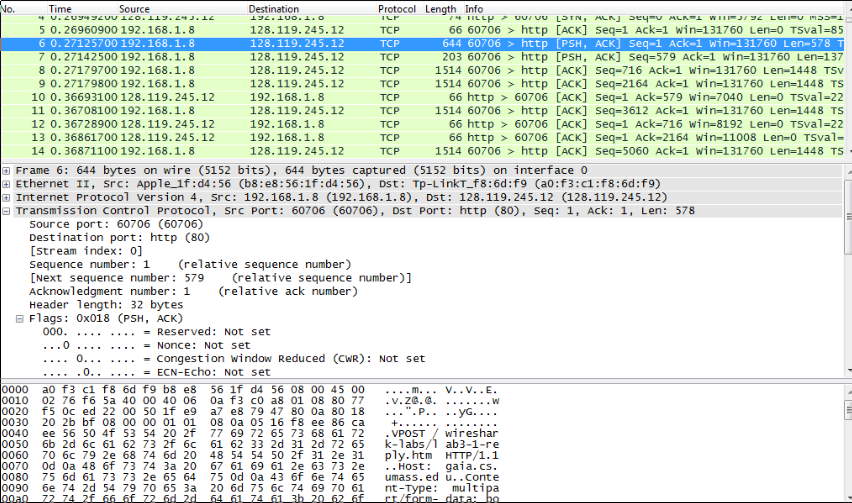
\includegraphics[scale=0.4]{Q7a.png}
\caption{First 6 segments}
\end{figure}

\begin{figure}[h!]
\centering
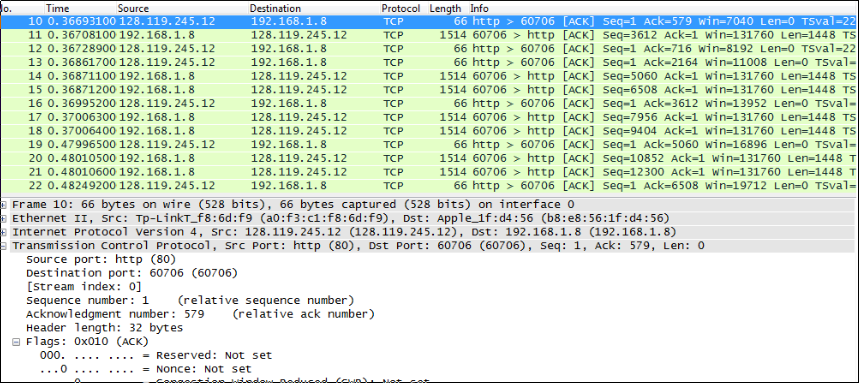
\includegraphics[scale=0.4]{Q7b.png}
\caption{First 6 segments ACKs}
\end{figure}

\begin{figure}[h!]
\centering
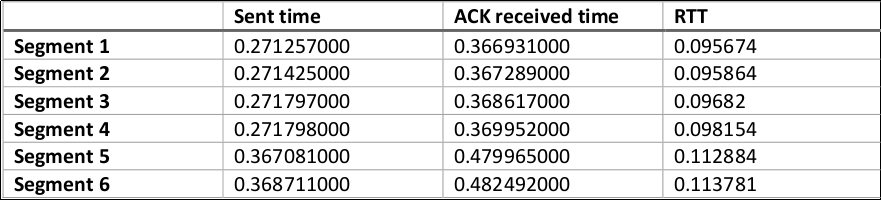
\includegraphics[scale=0.4]{Q7c.png}
\caption{Sending and receiving time of AKCs}
\end{figure}
\clearpage

\section*{8}
What is the length of each of the first six TCP segments?\\
\newline According to figure 8, the legnths of the first 6 segments are 74, 74, 66, 1514, 1514, 1514.\\
\begin{figure}[h!]
\centering
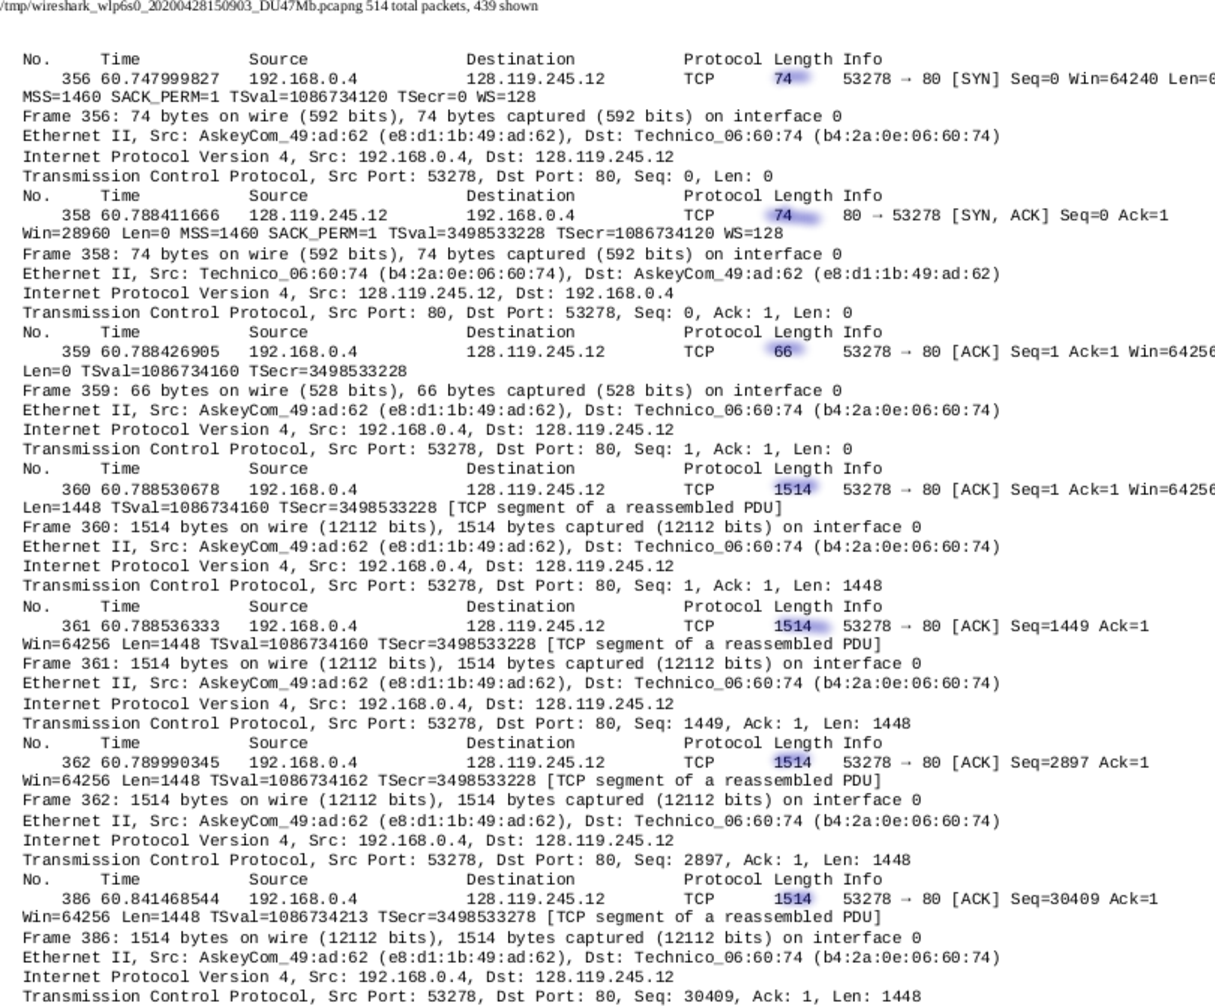
\includegraphics[scale=0.5]{Q8.pdf}
\caption{Length of each of the first six TCP segments}
\end{figure}
\section*{9}
What is the minimum amount of available buffer space advertised at the received
for the entire trace? Does the lack of receiver buffer space ever throttle the
sender?\\
\newline According to figure 9, the minimum amount of available buffer space advertised at the received
for the entire trace is 28960.  Throughout the trace, the window grows until it reaches a max buffer size.  Thus the sender is never throttled due to a lack of received buffer space.\\
\begin{figure}[h!]
\centering
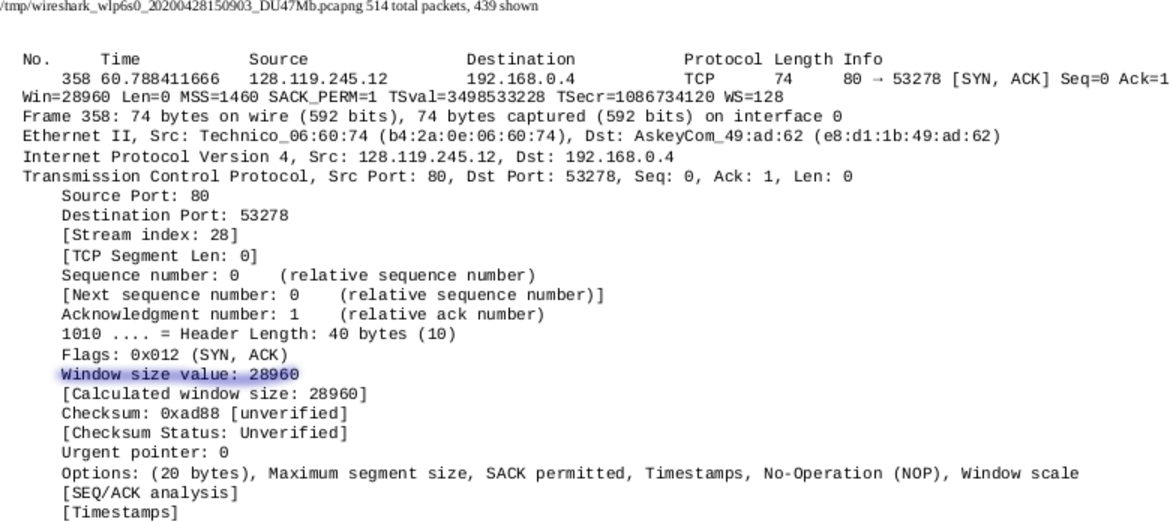
\includegraphics[scale=0.5]{Q9.pdf}
\caption{Minimum amount of available buffer space}
\end{figure}
\clearpage
\section*{10}
Are there any retransmitted segments in the trace file? What did you check for (in
the trace) in order to answer this question?\\
\newline According to figure 10, there are no retransmitted segments in the trace file. This can be checked by observing the sequence numbers of the TCP segments.  All the sequence numbers increase monotonically with respect to time.\\ 
\begin{figure}[h!]
\centering
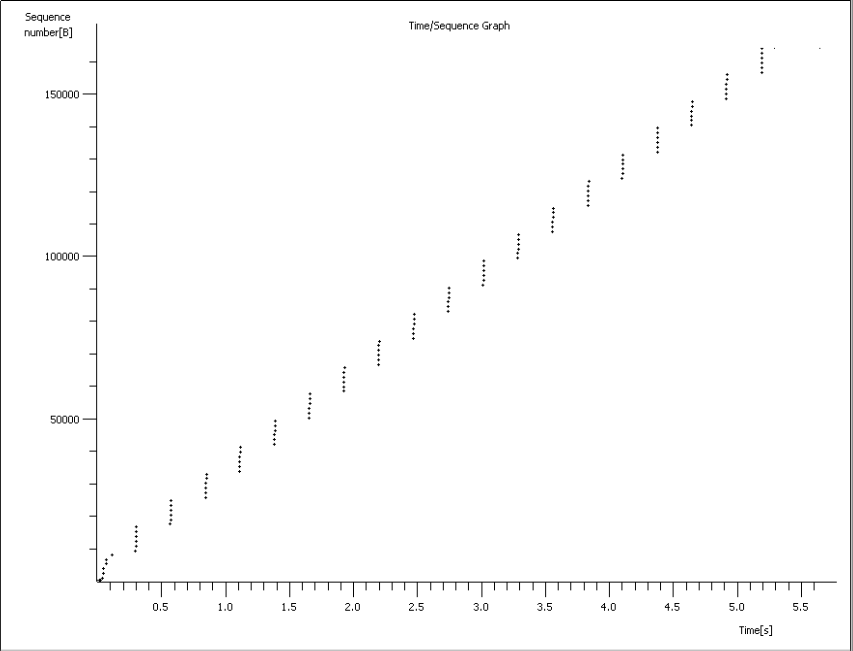
\includegraphics[scale=0.5]{Q13.png}
\caption{Time sequence graph}
\end{figure}
\clearpage

\section*{11}
How much data does the receiver typically acknowledge in an ACK? Can you
identify cases where the receiver is ACKing every other received segment (see
Table 3.2 on page 250 in the text).\\
\newline The amount of data being transfered can be found by observing the difference of the sequence numbers.  It typically acknowledges 1460.  According to the table, there are instances where the receiver is ACKing every other segment.\\
\begin{figure}[h!]
\centering
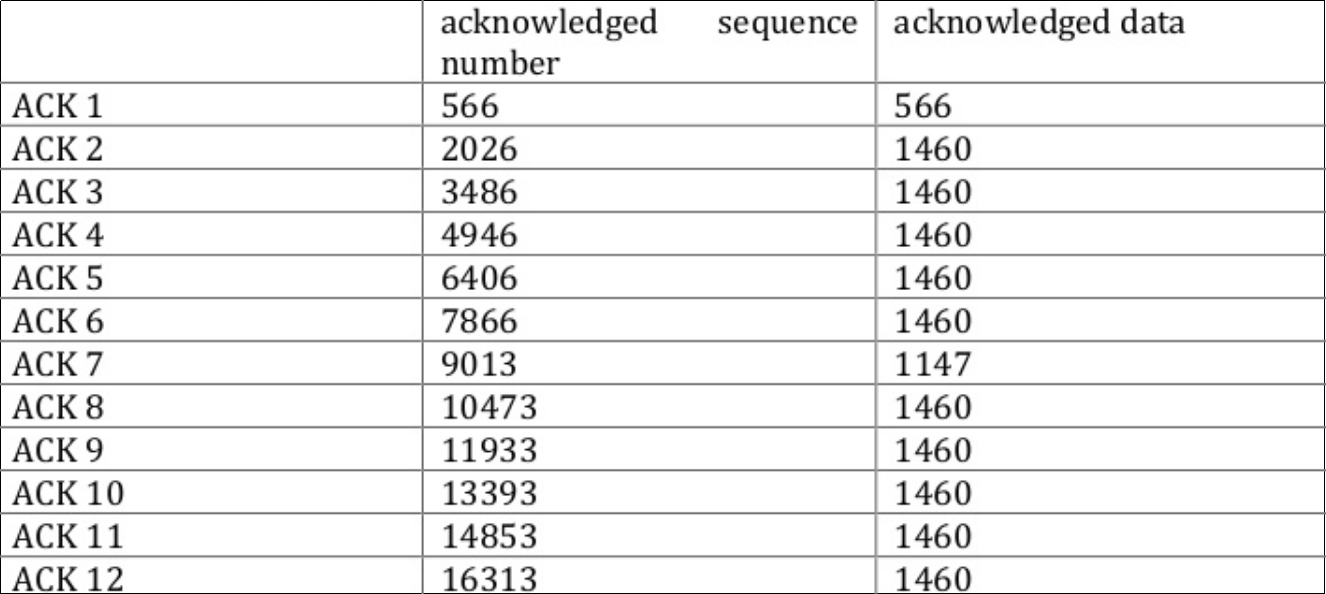
\includegraphics[scale=0.4]{Q11.png}
\caption{Table of ACK data}
\end{figure}
\section*{12}
What is the throughput (bytes transferred per unit time) for the TCP connection?
Explain how you calculated this value.\\
\newline The througput can be calculated by dividing the total data by the total time taken.  The total data is determined by finding the difference of the first and last sequence number. According to figure 12, the total time taken is $60.987296150 - 60.788426905 = 0.19886924$ and the difference of sequence numbers is $149362-1 = 149361$.  Thus the throughput is $\frac{149361}{0.19886924} = 751051.2938049$.\\
\begin{figure}[h!]
\centering
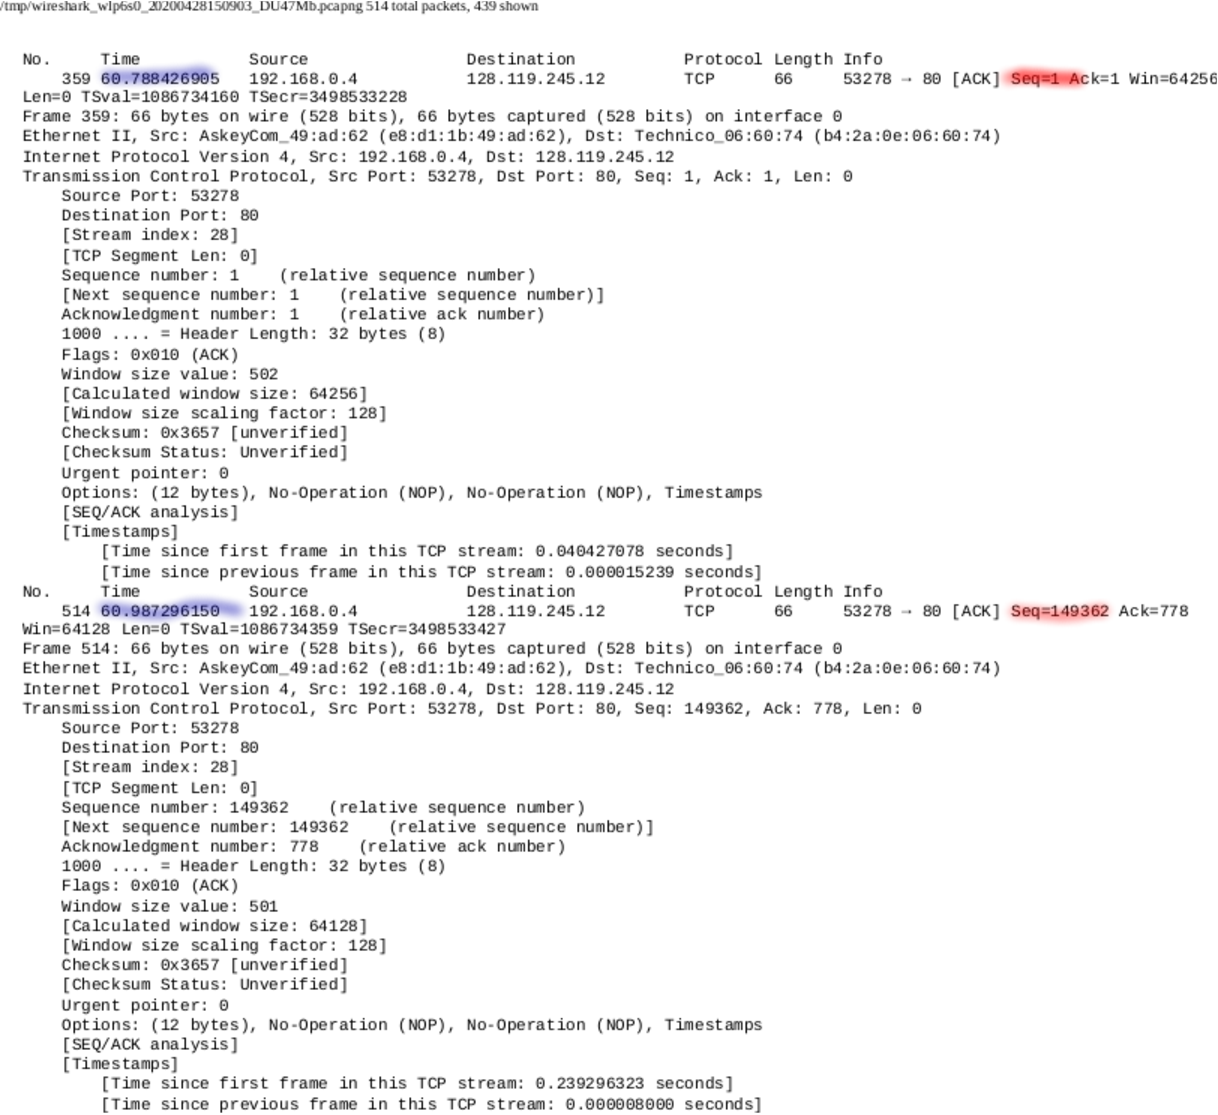
\includegraphics[scale=0.4]{Q12.pdf}
\caption{Firt and last packet data}
\end{figure}
\section*{13}
Use the Time-Sequence-Graph(Stevens) plotting tool to view the sequence
number versus time plot of segments being sent from the client to the
gaia.cs.umass.edu server. Can you identify where TCP’s slowstart phase begins
and ends, and where congestion avoidance takes over? Comment on ways in
which the measured data differs from the idealized behavior of TCP that we’ve
studied in the text.\\
\newline According to figure 13, TCP appears to begin at 0.27 seconds and ends at 10.35 seconds.  Congestion avoidance begins at about 0.7 seconds.  We know this is occuring because there is a reduced quantity of packets being disbatched.  We expect the sequence numbers to increase lineraly.  Here we can see that packets are sent in batches of 6, also, there is clearly non-linear behavior, especially at the start of the graph.\\
\begin{figure}[h!]
\centering
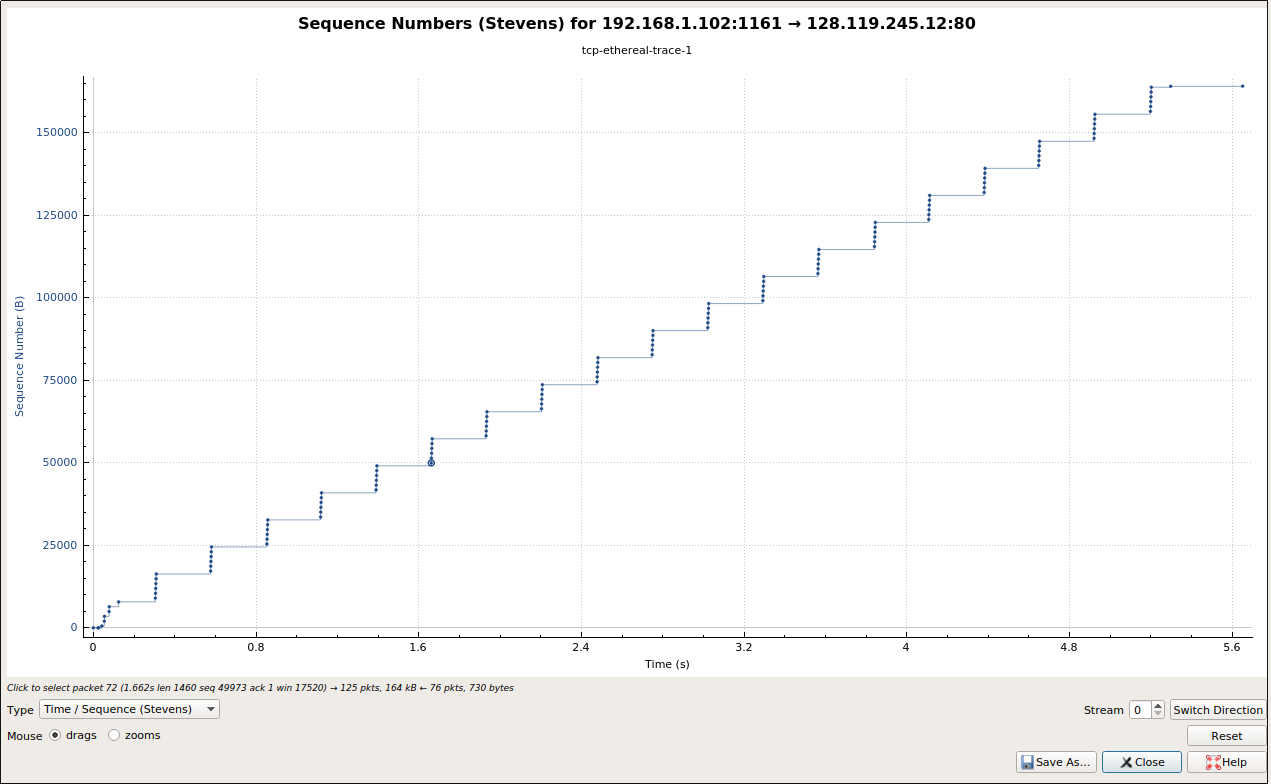
\includegraphics[scale=0.4]{Q13REAL.png}
\caption{Time sequence graph}
\end{figure}
\clearpage
\section*{14}
Answer each of two questions above for the trace that you have gathered when
you transferred a file from your computer to gaia.cs.umass.edu.\\
\newline According to figure 14, it appears to begin at 0.04 seconds and ends at 0.2 seconds.  Congestion avoidance begins at 0.8 seconds when it begins changing the window size.  This graph is more linear than the previous example with some gaps inbetween the batches.  The ideal case is a perfectly linear graph.\\
\newline According to figure 15, it appears to begin at 0.04 seconds and ends at 0.24 seconds.  Congestion avoidance begins at about 0.9 seconds when the window size begins to increase.  The figure does not resemble the ideal graph at all.  It has large spikes of sequence numbers and the flattens with the next batch.\\
\begin{figure}[h!]
\centering
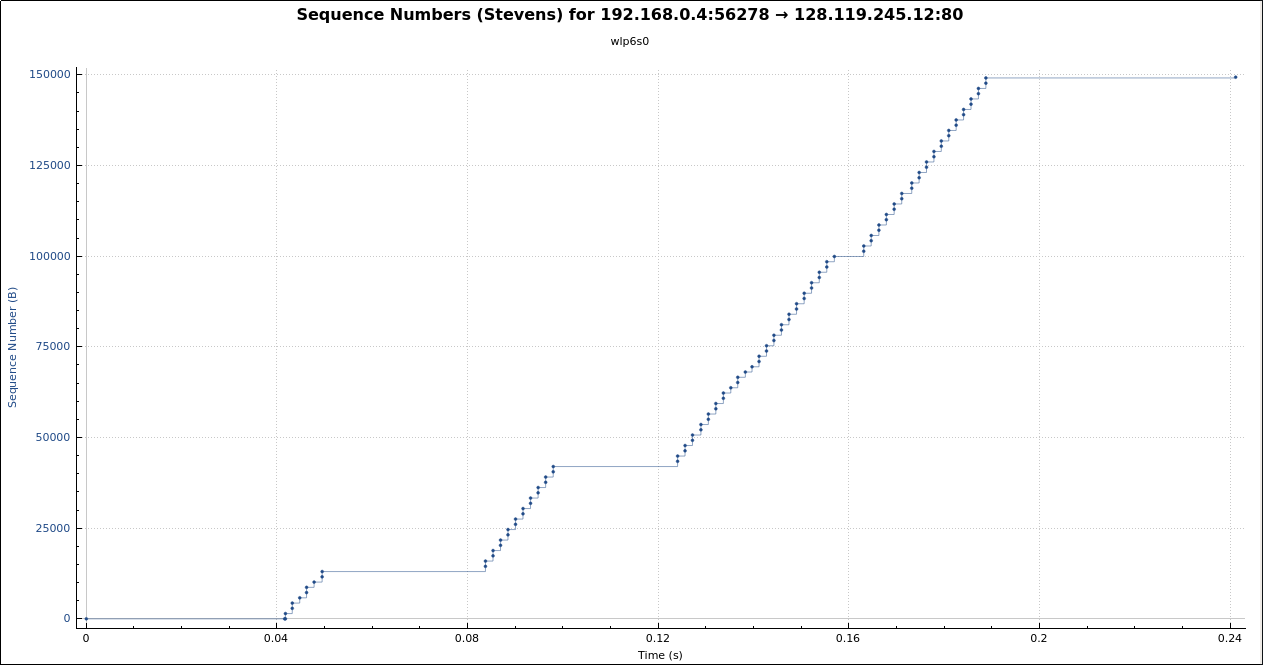
\includegraphics[scale=0.30]{Q14a.png}
\caption{Time sequence graph}
\end{figure}
\begin{figure}[h!]
\centering
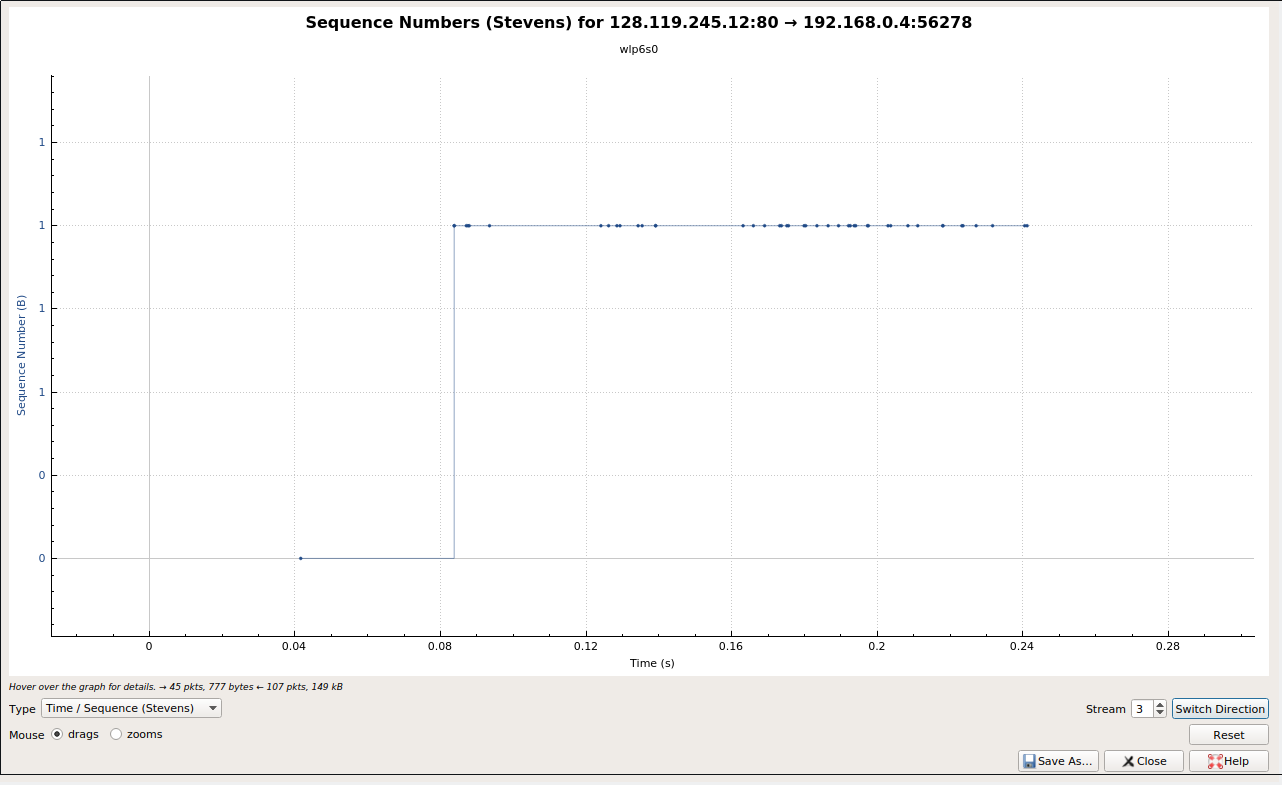
\includegraphics[scale=0.30]{Q14b.png}
\caption{Time sequence graph}
\end{figure}

\end{document}





% \begin{figure}[h!]
% \centering
% 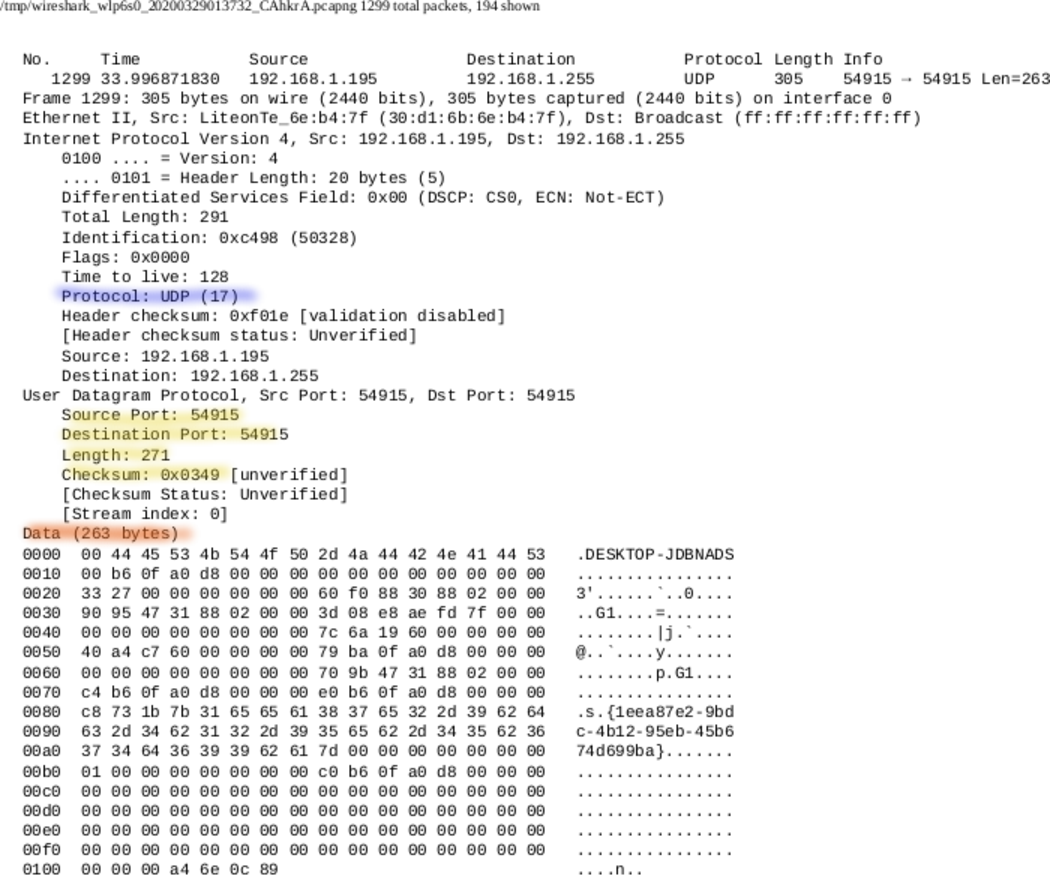
\includegraphics[scale=0.65]{Q1-7.pdf}
% \caption{}
% \end{figure}